\documentclass{exam}

\usepackage{units} 
\usepackage[fleqn]{amsmath}
\usepackage{float}
\usepackage{mdwlist}
\usepackage{booktabs}
\usepackage{caption}
\usepackage{fullpage}
\usepackage{enumerate}
\usepackage{graphicx}
\usepackage{2in1, lscape} 

\everymath{\displaystyle}

\author{}
\date{January 22, 2014}
\title{Statistics \\ Week One}

\begin{document}

  \maketitle

  \section{Data Sets}
  \begin{itemize*}
    \item {\em Observation} is one row
    \item Columns are {\em variables}
    \item Continuous variables are numbers that can take on any value
    \item Category variables are things like male/female, state, car model, etc.
  \end{itemize*}

  \section{Time Graphs}

  \subsection{Overview}

  Time graphs show how a continuous variable changes over time.  

  \begin{itemize*}
    \item x-axis is time
    \item y-axis is the quantity being measured
    \item can use line or bar
  \end{itemize*}

  \subsection{US}
  The total US population has been growing:
  \begin{figure}[H]
    \centering
    \includegraphics[scale = 0.9]{figures/us_population.eps}
    \caption{US population 1980 to 2010}
  \end{figure}

  so has the prison population:
  \begin{figure}[H]
    \centering
    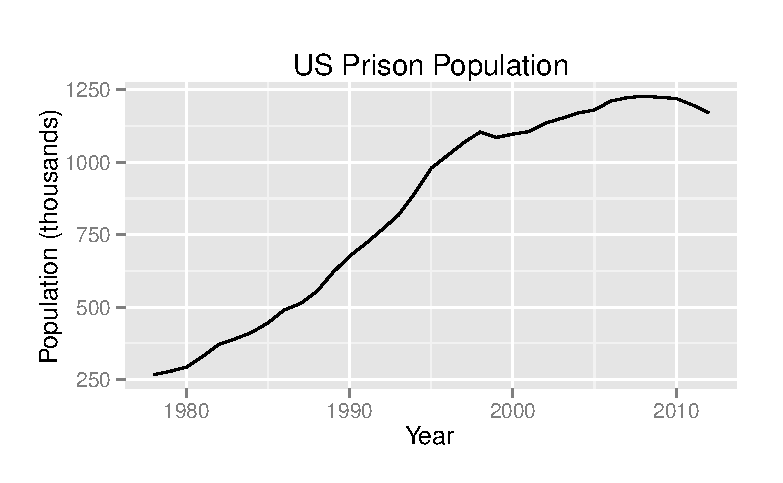
\includegraphics[scale = 0.9]{figures/us_prison_population.eps}
  \end{figure}

  You can make the US population growth look more impressive by changing the y-axis:
  \begin{figure}[H]
    \centering
    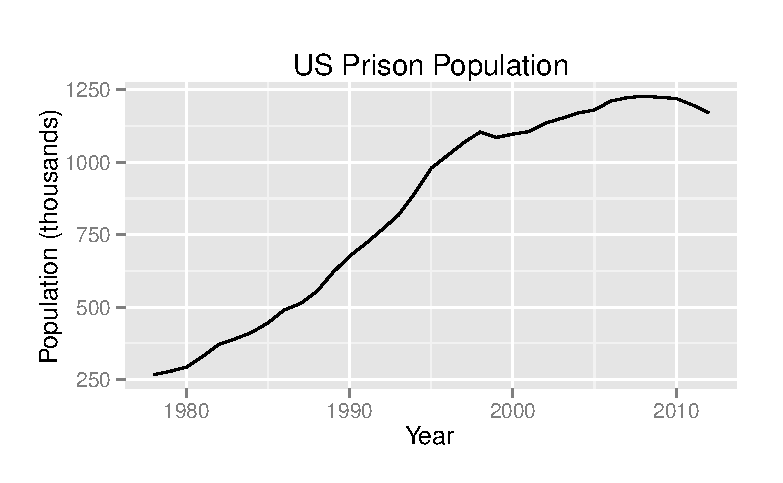
\includegraphics[scale = 0.9]{figures/us_prison_population.eps}
    \caption{US population with y-axis starting at 200}
  \end{figure}

  \subsection{Washington Graphs}

  \begin{figure}[H]
    \centering
    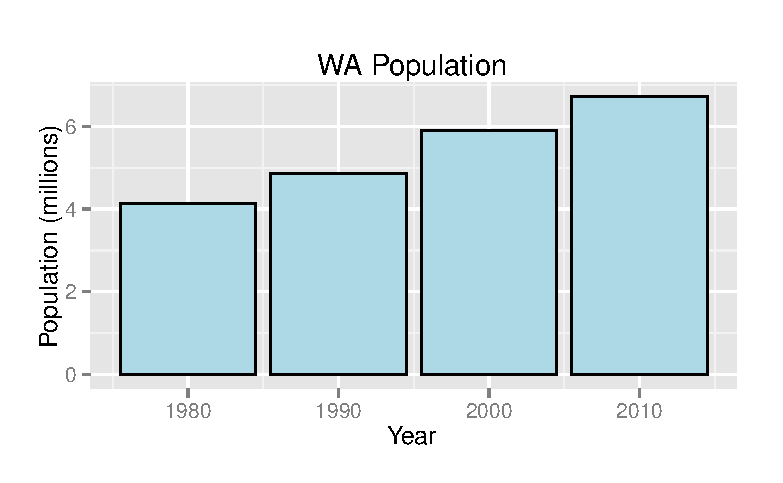
\includegraphics[scale = 0.9]{figures/wa_population.eps}
    \caption(WA population 1980-2010)
  \end{figure}

  \begin{figure}[H]
    \centering
    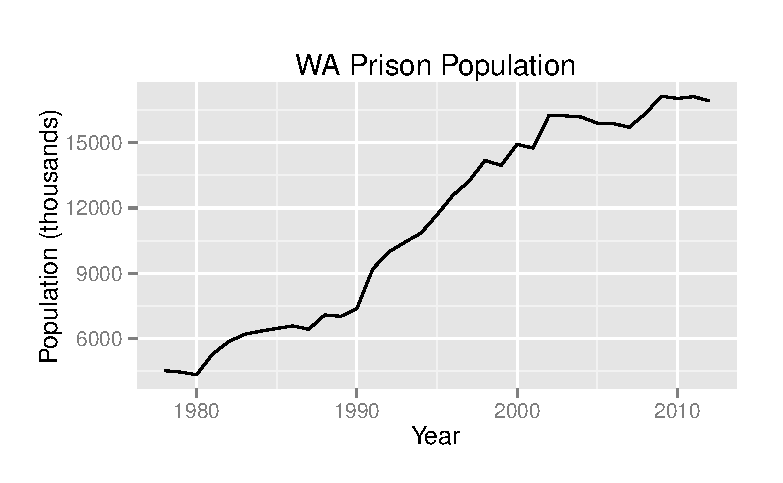
\includegraphics[scale = 0.9]{figures/wa_prison_population.eps}
    \caption(WA prison population 1980-2010)
  \end{figure}

  \subsection{State Prison Populations}
  \subsubsection{1980}
  \begin{figure}[H]
    \centering
    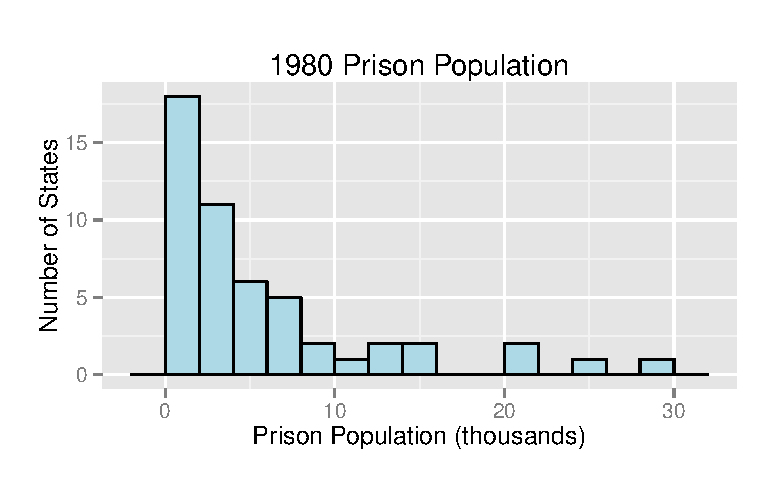
\includegraphics[scale = 0.9]{1980_pp_histogram.eps}
  \end{figure}

  \begin{figure}[H]
    \centering
    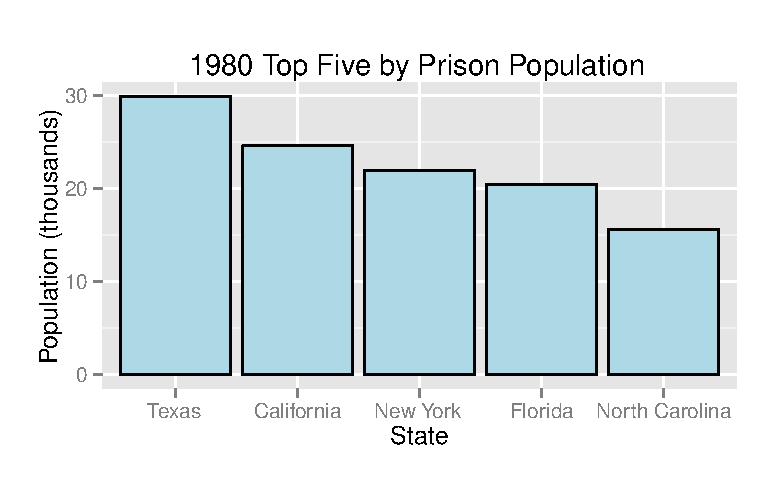
\includegraphics[scale = 0.9]{top_five_1980.eps}
  \end{figure}

  \subsubsection{2010}
  \begin{figure}[H]
    \centering
    \includegraphics[scale = 0.9]{2010_pp_histogram.eps}
  \end{figure}

  \begin{figure}[H]
    \centering
    \includegraphics[scale = 0.9]{top_five_2010.eps}
  \end{figure}

  \subsection{Top 5 2010 vs. 1980}
  \begin{figure}[H]
    \centering
    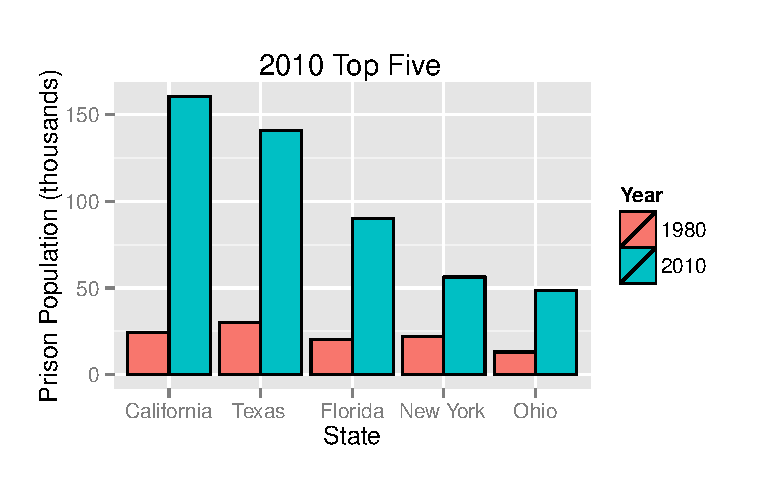
\includegraphics[scale = 0.9]{1980_to_2010_top_five.eps}
  \end{figure}

  \pagebreak

  \subsection{State Rates}

  \subsubsection{1980}
  \begin{itemize*}
    \item median 104
    \item mean 121
    \item highest rate was 265 (North Carolina)
    \item lowest rate was 34 (New Hampshire)
    \item highest population was 29,892 (Texas)
    \item lowest population was 313 (New Hampshire)
    \item skewed right
  \end{itemize*}

  \begin{figure}[H]
    \centering
    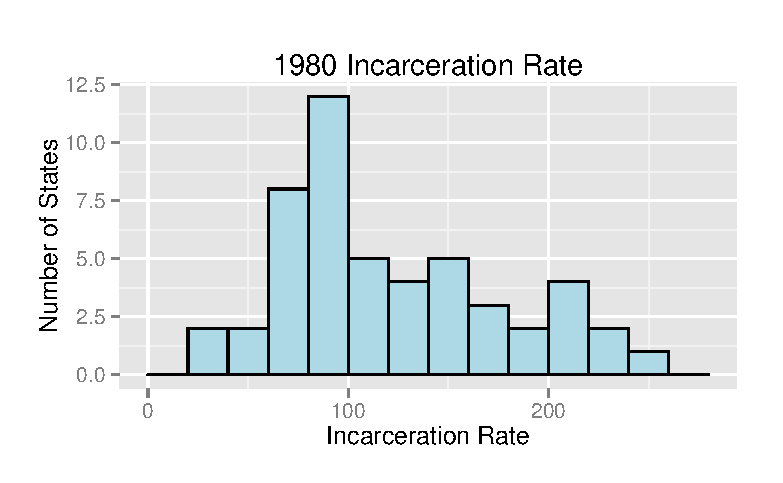
\includegraphics[scale = 0.9]{1980_rate_histogram.eps}
  \end{figure}

  \begin{figure}[H]
    \centering
    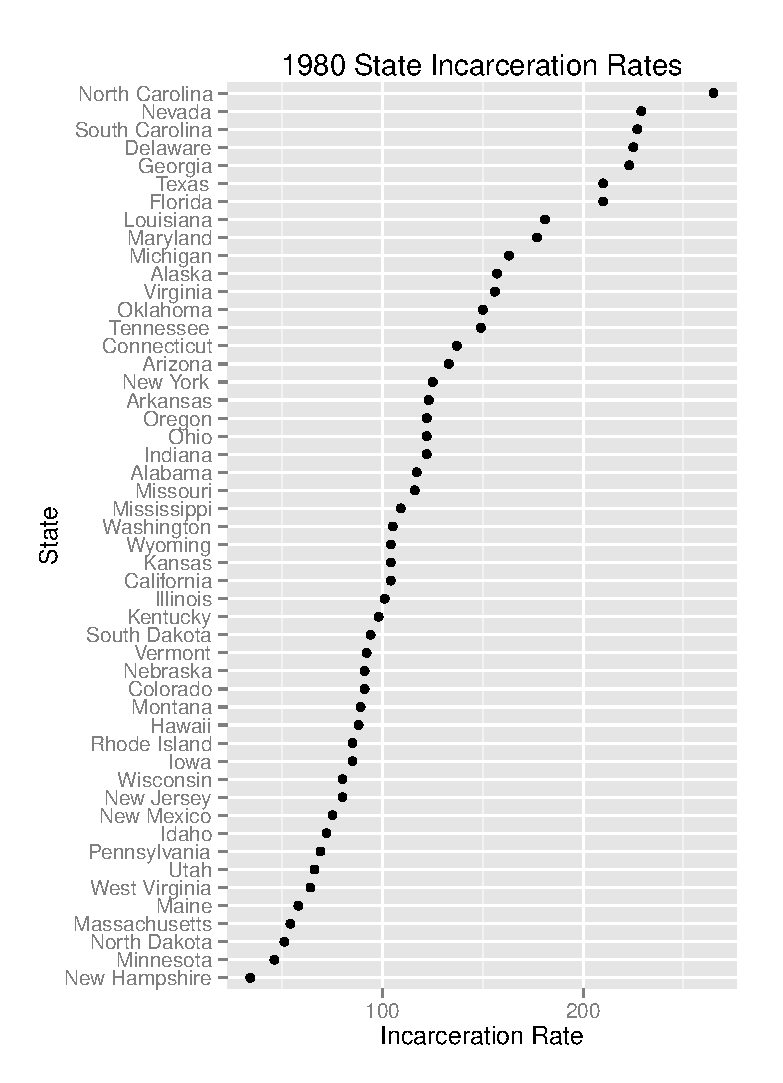
\includegraphics[scale = 0.9]{rate_by_state_1980.eps}
    \caption{1980 incarceration rates by state}
  \end{figure}

  \subsubsection{2010}
  \begin{itemize*}
    \item median rate 367
    \item mean rate 360
    \item highest rate was 710 (Delaware)
    \item lowest rate was 147 (Maine)
    \item highest population was 160,651 (California)
    \item lowest population was 1,416 (North Dakota)
    \item Delaware is outlier
    \item symmetric
  \end{itemize*}

  \begin{figure}[H]
    \centering
    \includegraphics[scale = 0.9]{2010_rate_histogram.eps}
  \end{figure}

  \begin{figure}[H]
    \centering
    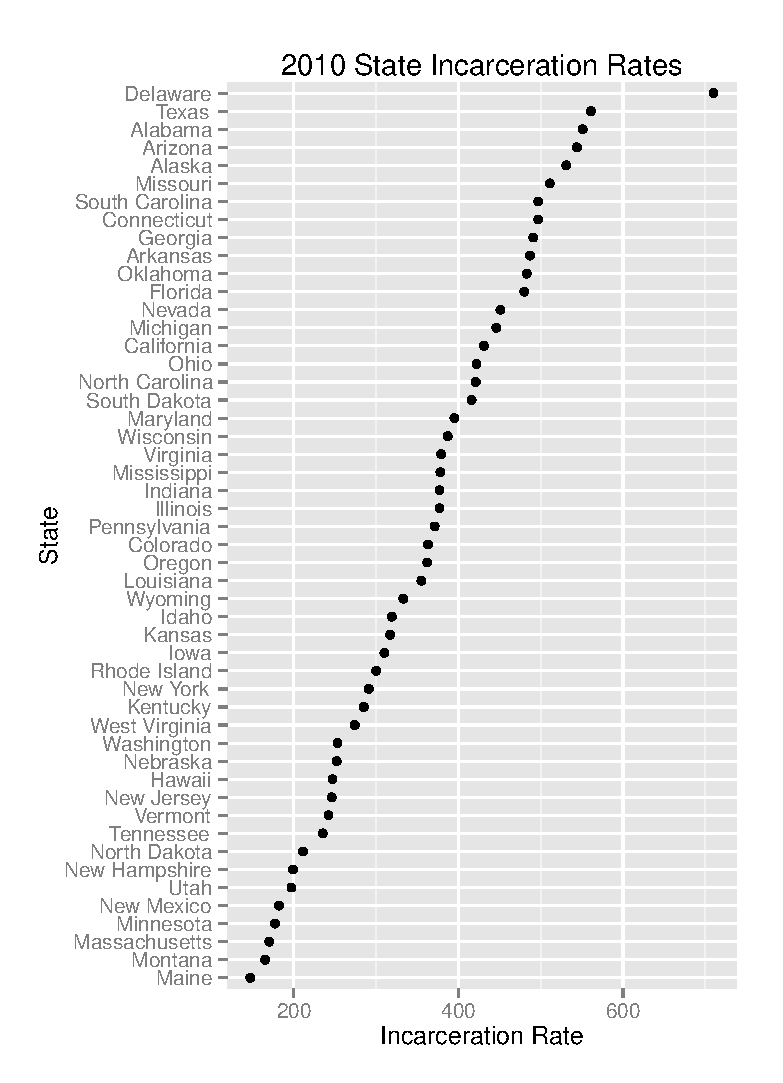
\includegraphics[scale = 0.9]{rate_by_state_2010.eps}
    \caption{2010 incarceration rates by state}
  \end{figure}

  \subsection{WA Rate over Time}
  \begin{figure}[H]
    \centering
    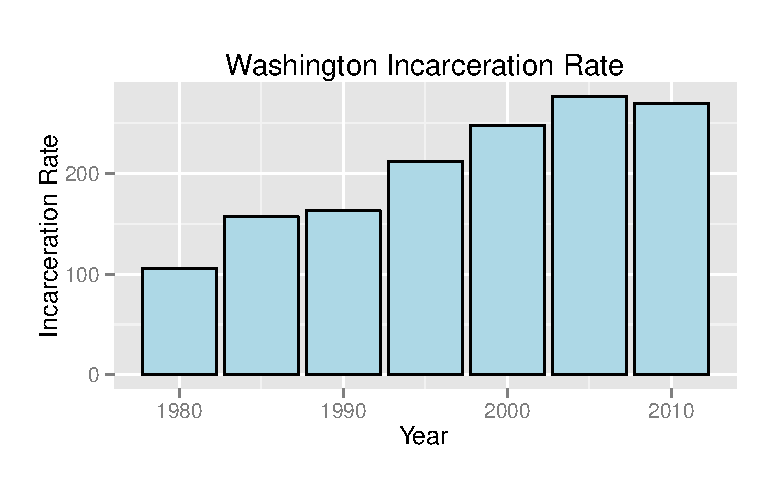
\includegraphics[scale = 0.9]{wa_rate.eps}
  \end{figure}

  \subsection{TX Rate over Time}
  \begin{figure}[H]
    \centering
    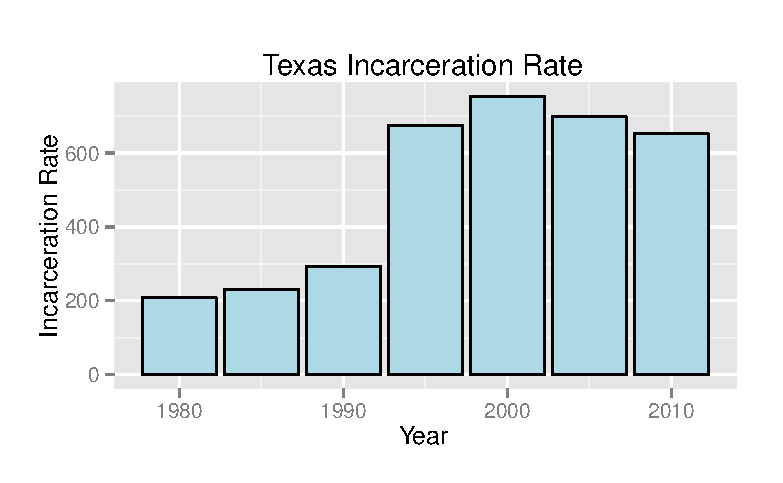
\includegraphics[scale = 0.9]{tx_rate.eps}
  \end{figure}

  \subsection{LA Rate over Time}
  \begin{figure}[H]
    \centering
    \includegraphics[scale = 0.9]{la_rate.eps}
  \end{figure}

  \subsection{Rates by Region}
  \begin{figure}[H]
    \centering
    \includegraphics[scale = 0.9]{rate_by_region.eps}
  \end{figure}

  \subsection{World Incarceration Rates}
  \begin{figure}[H]
    \centering
    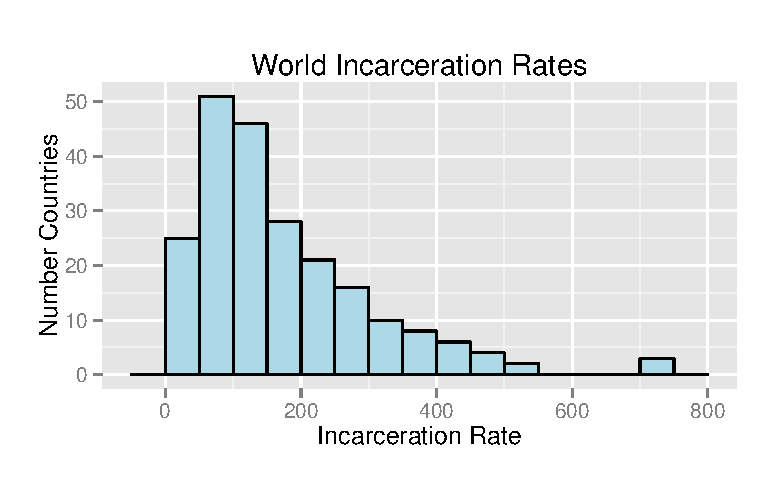
\includegraphics[scale = 0.9]{world_rate_histogram.eps}
  \end{figure}

  Median: 132

  \begin{figure}[H]
    \centering
    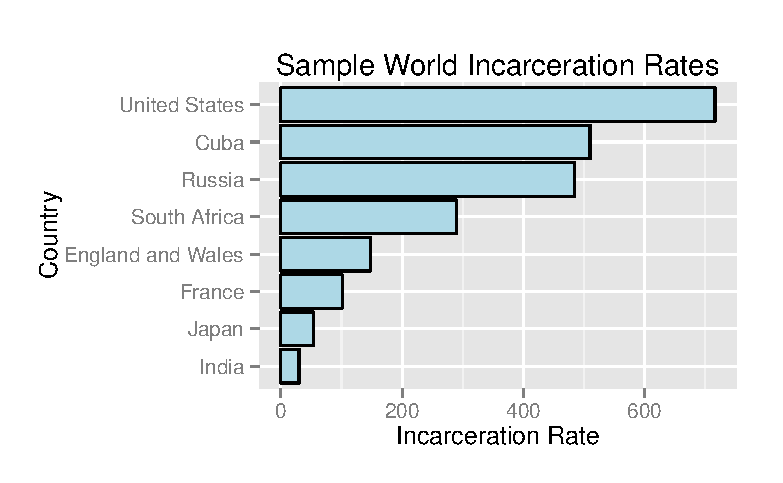
\includegraphics[scale = 0.9]{world_rates.eps}
  \end{figure}
\end{document}

